%-----------------begin---preamble-------------------
\documentclass{article}
\usepackage{amsmath,amssymb,amsthm}
\usepackage{tikz,tkz-euclide}
\usepackage{marginnote}
\usepackage{float}
\usepackage[margin=0.8in]{geometry}
% \usepackage{enumerate}


\usetikzlibrary{calc,patterns,angles,quotes}
\usetkzobj{all}

\def\deg{^{\circ}}
\def\thm{Th\textsuperscript{\underline{m}}}
\newcommand\heading[1]{\ \\\large{\textbf{#1}}}
\newcommand\ora[1]{\overrightarrow{#1}}

\newtheorem*{problem}{Problem}
%------------------end---preamble--------------------

\begin{document}
	\begin{problem}[Bulgarian National Mathematical Olympiad 2011, Problem 5]
		Isosceles $\triangle ABC\ (AC=BC)$ is inscribed in a circle $k$. A point $M$ lies on the side $BC$. A point $N$ from the ray $AM$ ($M$ lies between $A$ and $N$) is such that $AN=AC$. The circumcircle of $\triangle MCN$ intersects $k$ at $C$ and $P$, where $P$ is from the arc $BC$ not containing $A$. The lines $AB$ and $CP$ intersect at $Q$. Prove that $\angle QMB = \angle QMN$
	\end{problem}
	\begin{proof}
	\ \\Denote $\angle MAC=\alpha$ and $\angle ACB=\beta$. Let $J$ the incentre of $\triangle AMC$.
		\begin{figure}[H]
		\begin{center}
		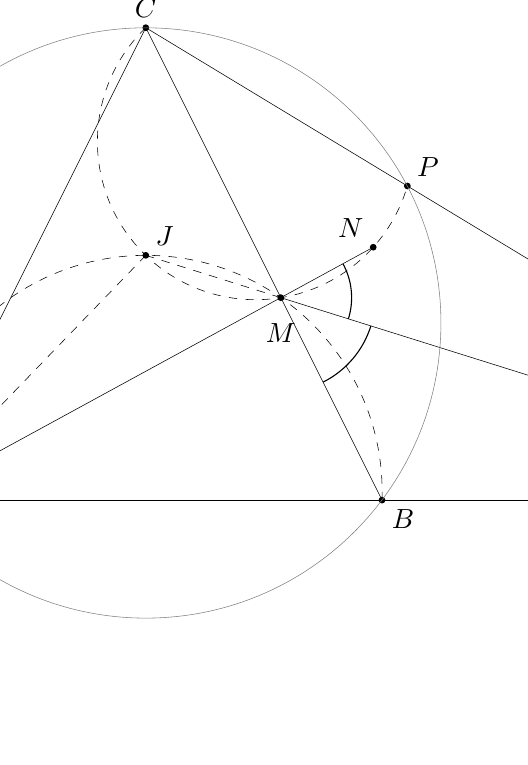
\begin{tikzpicture}[scale=3]
			\useasboundingbox (-.5,-1) rectangle  (1.5,2);
			\tkzDefPoint(-1,0){A}
			\tkzDefPoint(1,0){B}
			\tkzDefPoint(0,2){C}
			\tkzDefCircle[circum](A,B,C)\tkzGetPoint{O}
			\tkzDefBarycentricPoint(C=3,B=4)\tkzGetPoint{M}
			\tkzInterLC(A,M)(A,C)\tkzGetSecondPoint{N}
			\tkzDefCircle[circum](M,N,C)\tkzGetPoint{I}
			\tkzInterCC(I,C)(O,C)\tkzGetFirstPoint{P}
			\tkzInterLL(C,P)(A,B)\tkzGetPoint{Q}
			\tkzDefCircle[in](A,M,C)\tkzGetPoint{J}

			\tkzDrawPoints[fill=black](A,B,C,M,N,P,Q,J)
			\tkzDrawSegments(A,Q B,C C,A A,N C,Q M,Q)
			\tkzDrawSegments[dashed](A,J J,M)
			\tkzMarkAngle[size=0.3](Q,M,N)
			\tkzMarkAngle[size=0.4](B,M,Q)

			\tkzDrawArc[rotate,dashed,color=black](I,C)(210)
			\tkzDefCircle[circum](A,B,M)\tkzGetPoint{K}\tkzGetLength{r}
			\tkzDrawArc[rotate,dashed,color=black](K,B)(185)
			\tkzDrawCircle(O,A)
			\tkzLabelPoints[above](C)
			\tkzLabelPoints[below=0.2](M)
			\tkzLabelPoints[below left](A,Q)
			\tkzLabelPoints[below right](B)
			\tkzLabelPoints[above right](J,P)
			\tkzLabelPoints[above left](N)


			
			\end{tikzpicture}
		\end{center}		
		\end{figure}
	 It follows that $\angle AJM=90\deg+\beta/2$ and $\angle ABM=90\deg- \beta/2$, which implies that the quadrilateral $ABMJ$ is inscribed in a circle $k_1$. Analogously we have that the quadrilateral $MNCJ$ is inscribed in a circle $k_2$ which is just the circumcircle of $\triangle MCN$. Therefore $P$ is a point on $k_2$. Since $QA \cdot QB =QC \cdot QP$ we conclude that $Q$ lies on $JM$, which is the angle bisector of $\angle BNC$. Thus $\angle QMB = \angle QMN$
	\end{proof}

	
	
\end{document}
